% Ejercicio 9, inciso d) — issue #4. Mismo contenido que inciso-d.md.
% Fragmento sin preámbulo: lo incluye latex/main.tex, que ya pone el título del inciso.

\begin{quote}
\itshape
Evalúa el rendimiento con 1M de clientes. ¿Cómo cambia el orden de complejidad? Propón
Observer con Thread Pool o Reactive Streams.
\end{quote}

Este inciso mide el código del inciso b con la entrega asíncrona del inciso c, propone una
alternativa indexada y la mide junto a la versión ingenua.

\begin{lstlisting}[language={}, numbers=none, basicstyle=\ttfamily\footnotesize, columns=fullflexible, keepspaces=true]
cd codigo
dotnet run -c Release --project Bolsa.Notificaciones -- rendimiento        # hasta 1 000 000
dotnet run -c Release --project Bolsa.Notificaciones -- rendimiento 100000 # más rápido
dotnet test                                                                # 27 pruebas
\end{lstlisting}

\textbf{Importante:} \texttt{-c Release}. En \texttt{Debug} el compilador no optimiza y los
tiempos no significan nada.

\begin{table}[H]
\centering
\small
\begin{tabularx}{\textwidth}{>{\raggedright\arraybackslash}p{4.1cm} >{\raggedright\arraybackslash}X}
\toprule
\textbf{Pregunta} & \textbf{Respuesta} \\
\midrule
¿Cómo se comporta con 1M de clientes? &
Un solo cambio de precio tarda \textbf{112,3\,ms} recorriendo las alertas una por una, y
ocupa \textbf{244\,MB}. Con 5 acciones cotizando cada segundo, la detección sola consume más
de medio segundo por segundo: el sistema no llega. \\
\addlinespace
¿Cómo cambia el orden de complejidad? &
La versión ingenua es $\Theta(n)$ por cambio de precio: revisa los $n$ umbrales aunque solo
haya que avisar a $k$ clientes. Ordenando los umbrales, los cruzados son un \textbf{tramo
contiguo} que se localiza con dos búsquedas binarias: $O(\log n + k)$. Medido:
112,3\,ms $\rightarrow$ \textbf{0,154\,ms} (731$\times$). \\
\addlinespace
¿Thread Pool o Reactive Streams? &
\textbf{Las dos cosas, en sitios distintos:} un pool de consumidores para repartir los $k$
envíos (medido: 6\,409 avisos/s con 8 consumidores frente a 792 con uno), y una \textbf{cola
acotada} (\texttt{System.Threading.Channels}) para el \emph{backpressure}. Rx.NET no sirve
para lo segundo, y se explica por qué. \\
\bottomrule
\end{tabularx}
\caption{Las respuestas en corto.}
\end{table}

\subsubsection{Cómo se midió}

\begin{itemize}
  \item \textbf{\texttt{Stopwatch}}, no BenchmarkDotNet: la unidad que interesa no es una
        función aislada sino \emph{un cambio de precio sobre una estructura de $n$
        suscripciones}, que hay que construir antes y que ocupa cientos de megabytes.
        BenchmarkDotNet habría dado más rigor estadístico a costa de no poder medir eso.
  \item \textbf{Mediana de 11 ticks}, descartando 3 de calentamiento. La mediana y no la
        media: una pausa del recolector de basura en un solo tick desplazaría la media.
  \item \textbf{Canales simulados sin E/S real} (\texttt{CanalSilencioso}, que solo cuenta).
        Escribir en la consola cuesta más que el envío simulado y falsearía la medición.
  \item \textbf{Las dos fases se miden por separado}, porque solo una cambia de orden:
        \emph{detectar} a quién avisar y \emph{entregar} los avisos.
  \item \textbf{Semillas y umbrales deterministas:} el benchmark es reproducible.
\end{itemize}

\textbf{Máquina:} Intel Core i5-7300U a 2,60\,GHz (2 núcleos, 4 hilos), 15\,GiB de RAM,
Garuda Linux x64 (kernel 7.2.11-zen), .NET SDK 10.0.113 / runtime 10.0.13, GC de estación de
trabajo.

\paragraph{Los dos escenarios.}
El resultado depende por completo de \textbf{cuántos clientes hay que avisar de verdad} en
cada tick, así que se miden los dos extremos.

\begin{table}[H]
\centering
\small
\begin{tabularx}{\textwidth}{>{\raggedright\arraybackslash}p{3.1cm} >{\raggedright\arraybackslash}X >{\raggedright\arraybackslash}p{4.3cm}}
\toprule
\textbf{Escenario} & \textbf{Cómo se reparten los umbrales} & \textbf{$k$ por tick} \\
\midrule
A · dispersos & un umbral por centavo (densidad fija); con más clientes, la banda de precios cubierta es más ancha & \textbf{constante}: 50, no importa cuánto crezca $n$ \\
\addlinespace
B · concentrados & los $n$ umbrales repartidos en una banda fija de 30\,\$ alrededor del precio & \textbf{proporcional a $n$}: $n/100$ \\
\bottomrule
\end{tabularx}
\caption{Ninguno es «el realista»: el real está en medio, y por eso interesa ver los dos.}
\end{table}

\subsubsection{Resultados}

\begin{figure}[H]
  \centering
  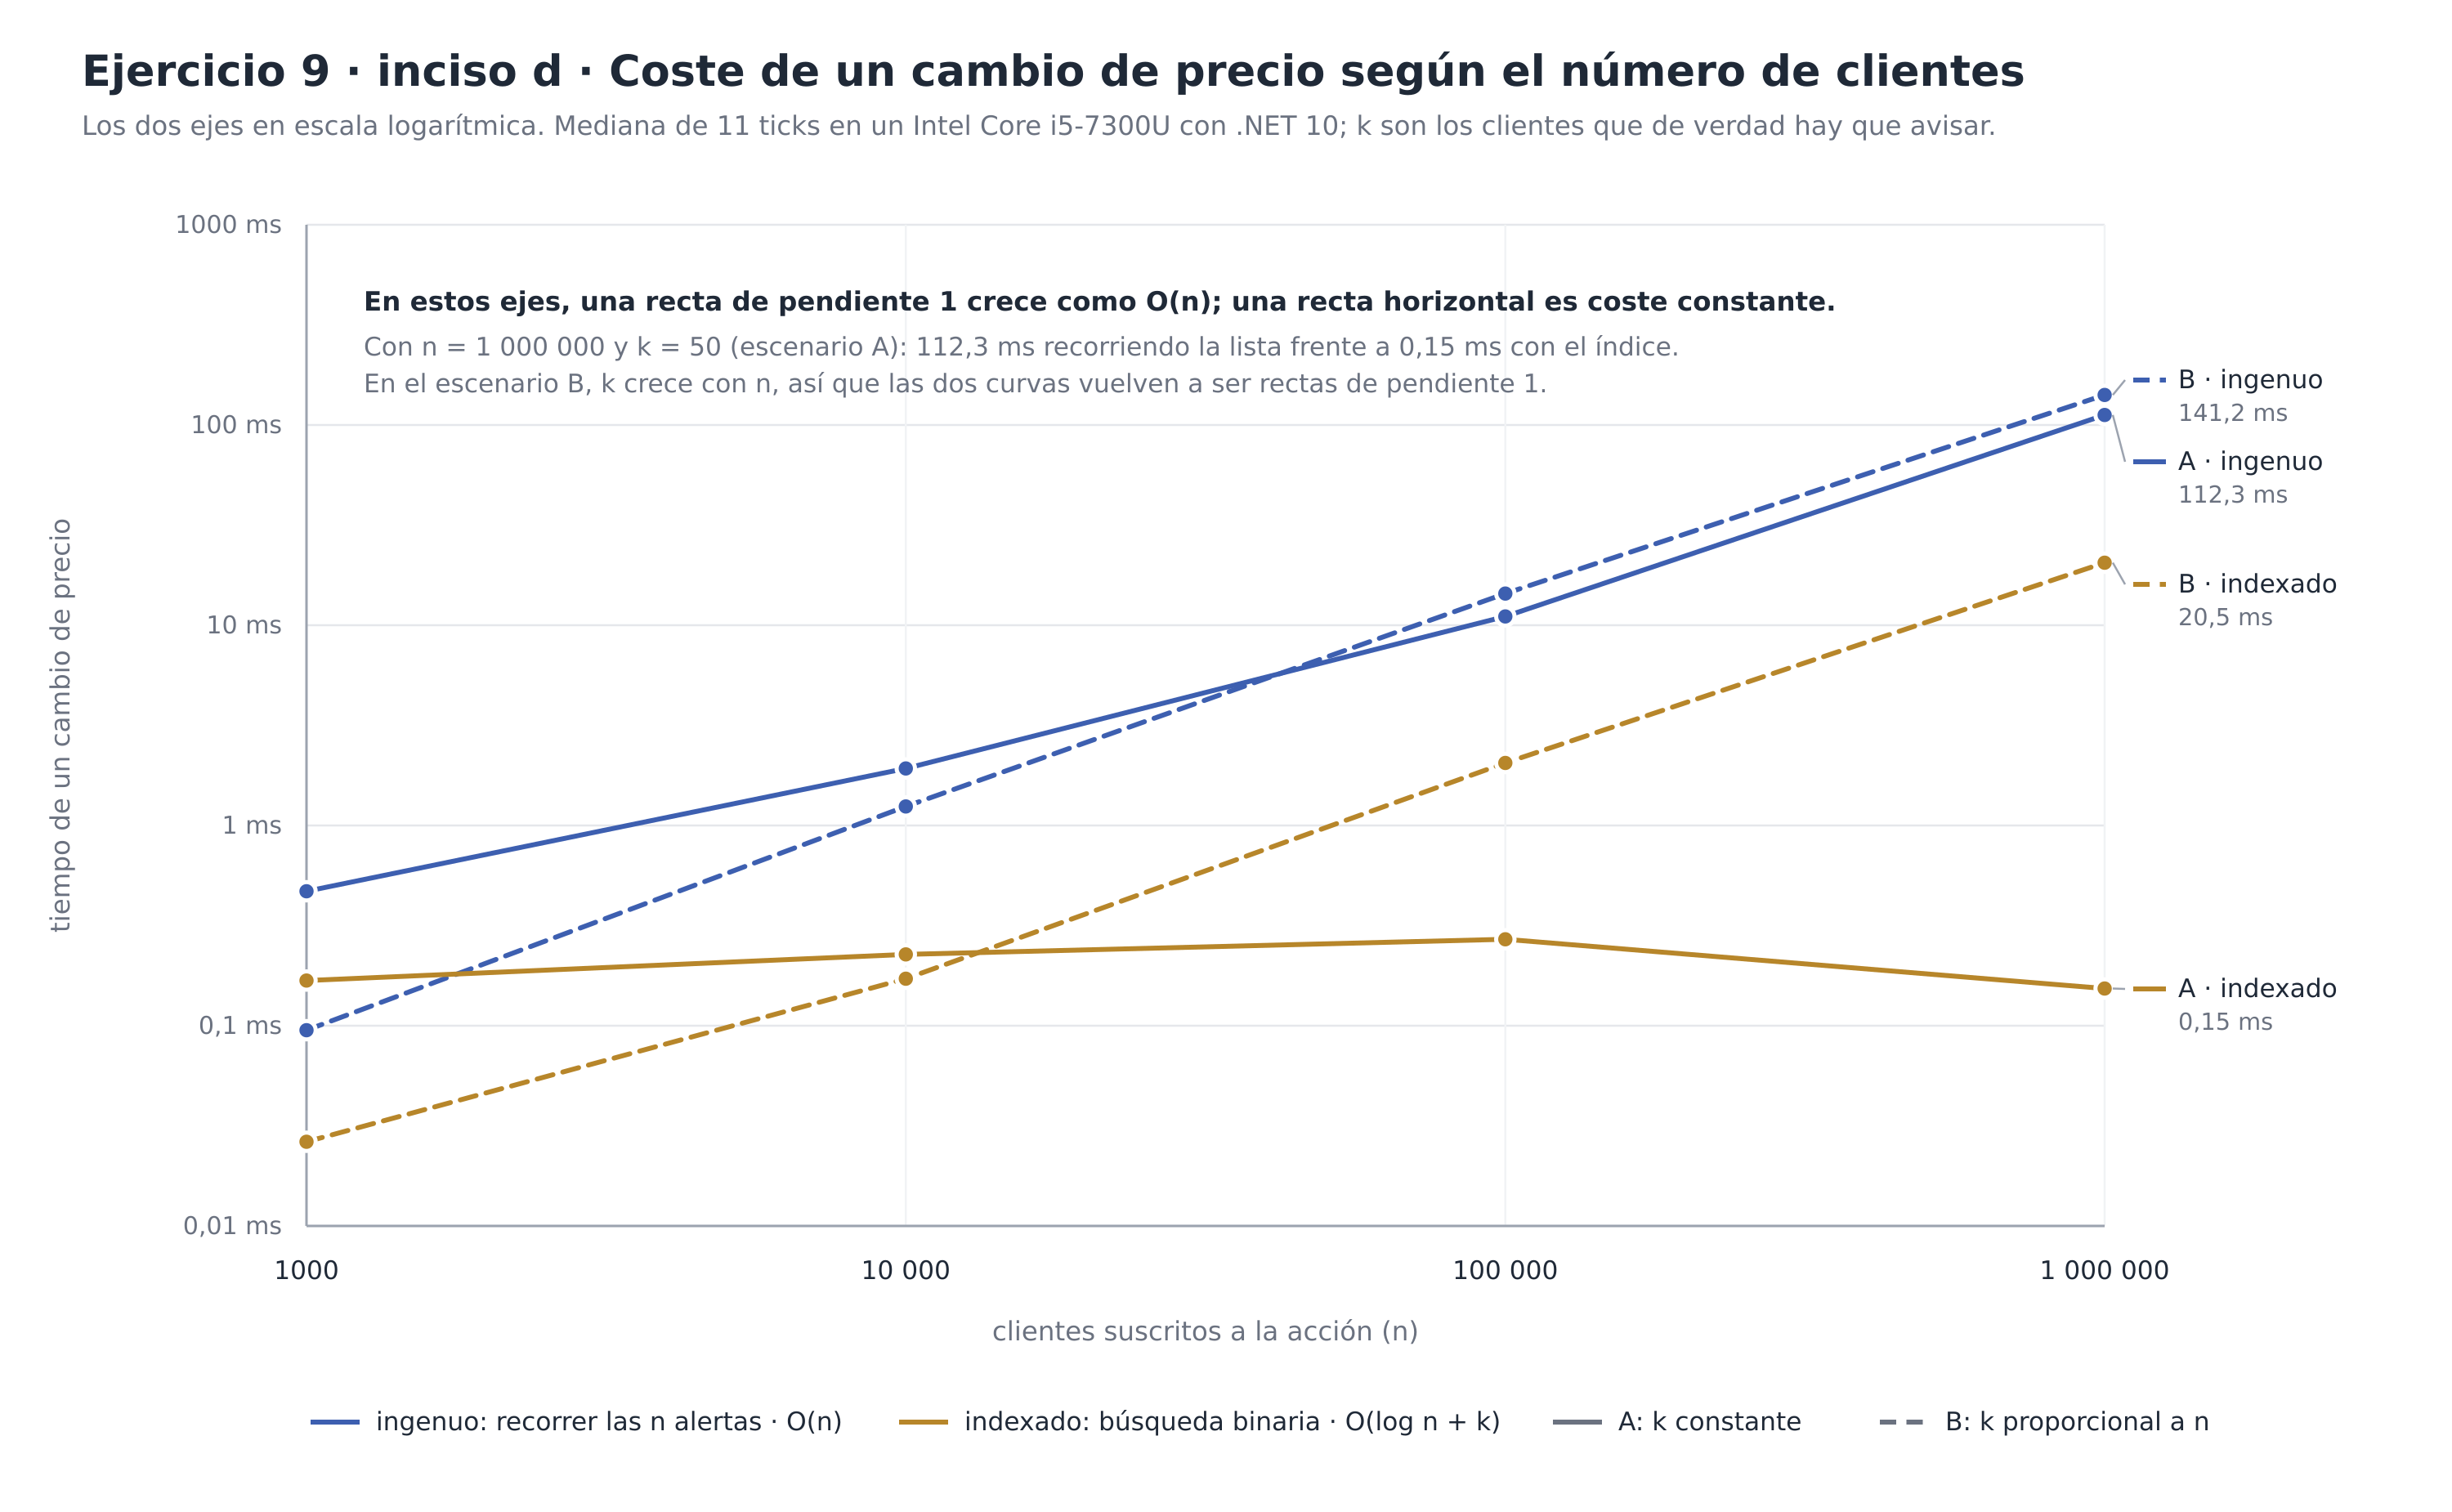
\includegraphics[width=\textwidth]{ejercicio-09-notificaciones-bolsa/diagramas/inciso-d-escalado.png}
  \caption{El recorrido ingenuo es una recta de pendiente 1 (crece como $n$); el índice con
  $k$ constante es una recta horizontal.}
  \label{fig:e9-escalado}
\end{figure}

\begin{table}[H]
\centering
\small
\begin{tabular}{rrrrrrr}
\toprule
\textbf{n} & \textbf{k} & \textbf{Ingenuo} & \textbf{Indexado} & \textbf{Mejora} & \textbf{Memoria} & \textbf{Construcción} \\
\midrule
1\,000 & 50 & 0,469\,ms & 0,168\,ms & 2,8$\times$ & 0,2 / 0,2\,MB & 2 / 1\,ms \\
10\,000 & 50 & 1,925\,ms & 0,227\,ms & 8,5$\times$ & 2,4 / 1,8\,MB & 40 / 47\,ms \\
100\,000 & 50 & 11,068\,ms & 0,270\,ms & 41,0$\times$ & 24,4 / 17,7\,MB & 577 / 169\,ms \\
\textbf{1\,000\,000} & 50 & \textbf{112,275\,ms} & \textbf{0,154\,ms} & \textbf{731,4$\times$} & 244,1 / 174,8\,MB & 2\,652 / 1\,108\,ms \\
\bottomrule
\end{tabular}
\caption{Escenario A: umbrales dispersos ($k = 50$ constante). Memoria y construcción:
ingenuo / indexado.}
\end{table}

El ingenuo multiplica su tiempo por 10 cada vez que $n$ se multiplica por 10: eso \emph{es}
$\Theta(n)$. El indexado se queda entre 0,15 y 0,27\,ms en todo el rango. Las diferencias
entre esos cuatro valores son ruido de medición, no crecimiento; lo que domina ahí no es el
$\log n$ (20 comparaciones) sino crear los 50 mensajes.

\begin{table}[H]
\centering
\small
\begin{tabular}{rrrrrrr}
\toprule
\textbf{n} & \textbf{k} & \textbf{Ingenuo} & \textbf{Indexado} & \textbf{Mejora} & \textbf{Memoria} & \textbf{Construcción} \\
\midrule
1\,000 & 10 & 0,095\,ms & 0,026\,ms & 3,6$\times$ & 0,2 / 0,2\,MB & 1 / 1\,ms \\
10\,000 & 100 & 1,245\,ms & 0,172\,ms & 7,3$\times$ & 2,4 / 1,7\,MB & 12 / 5\,ms \\
100\,000 & 1\,000 & 14,383\,ms & 2,054\,ms & 7,0$\times$ & 24,4 / 16,8\,MB & 252 / 63\,ms \\
\textbf{1\,000\,000} & 10\,000 & \textbf{141,246\,ms} & \textbf{20,510\,ms} & \textbf{6,9$\times$} & 244,1 / 167,8\,MB & 2\,879 / 1\,015\,ms \\
\bottomrule
\end{tabular}
\caption{Escenario B: umbrales concentrados ($k = n/100$). La mejora se estanca en
$\sim$7$\times$.}
\end{table}

Aquí la mejora \textbf{no crece con $n$}. No es un fallo del índice: cuando $k$ es
proporcional a $n$, el término $k$ domina y $O(\log n + k)$ \emph{también} es $\Theta(n)$. El
índice sigue ganando, pero por una constante (se ahorra tocar los 990\,000 clientes que no
cruzaron), no por un orden.

\begin{quote}
\textbf{La lección del par de tablas:} el índice no ``hace rápido'' el sistema. Elimina el
trabajo inútil ---mirar umbrales que no se cruzaron--- y deja solo el trabajo inevitable:
atender a los $k$ clientes que sí hay que avisar.
\end{quote}

\subsubsection{¿Cómo cambia el orden de complejidad?}

\paragraph{La versión ingenua: $\Theta(n)$ por cambio de precio.}
Por cada cambio de precio de una acción se recorren \textbf{todos} sus observadores, se cruce
su umbral o no. Si esa acción tiene $n$ suscripciones, el costo es $\Theta(n)$, y sumando el
trabajo de los $k$ que sí cruzan, $\Theta(n + k) = \Theta(n)$, porque $k \le n$.

Con 1\,000\,000 de clientes y un tick por segundo en 5 acciones, eso es \textbf{5\,000\,000
de comprobaciones por segundo} para, en el escenario A, avisar a 250 personas. El 99,99\,\%
del trabajo se tira.

\paragraph{La versión indexada: $O(\log n + k)$.}
La clave está en que la regla de disparo del inciso b es un \textbf{predicado de intervalo}:
\texttt{Sube} notifica si el umbral está en $[\text{anterior}, \text{nuevo})$, y
\texttt{Baja} si está en $(\text{nuevo}, \text{anterior}]$. Si los umbrales están
\textbf{ordenados}, los que cumplen esa condición forman un \textbf{tramo contiguo} del
array, y localizar sus dos extremos es una búsqueda binaria cada uno.

\begin{lstlisting}[basicstyle=\ttfamily\footnotesize, columns=fullflexible, keepspaces=true, caption={\texttt{GestorUmbralesIndexado}: dos búsquedas binarias y el recorrido del tramo.}]
public void Actualizar(CambioPrecio cambio)
{
    if (cambio.PrecioNuevo > cambio.PrecioAnterior)
    {
        Avisar(
            _umbralesSube,
            _clientesSube,
            PrimeroMayorOIgual(_umbralesSube, cambio.PrecioAnterior),  // O(log n)
            PrimeroMayorOIgual(_umbralesSube, cambio.PrecioNuevo),     // O(log n)
            Direccion.Sube,
            cambio);
    }
    else if (cambio.PrecioNuevo < cambio.PrecioAnterior)
    {
        // Una bajada solo puede cruzar umbrales "Baja", y al revés.
        Avisar(_umbralesBaja, _clientesBaja,
            PrimeroMayor(_umbralesBaja, cambio.PrecioNuevo),
            PrimeroMayor(_umbralesBaja, cambio.PrecioAnterior),
            Direccion.Baja, cambio);
    }
}
\end{lstlisting}

\paragraph{Esto no rompe el patrón: el índice es un ChangeManager.}
Podría parecer que indexar los umbrales obliga al sujeto a conocer a los clientes, que es
justo lo que el inciso a evitaba. No es así: el índice vive \textbf{dentro de un único
observador}.

\begin{lstlisting}[basicstyle=\ttfamily\footnotesize, columns=fullflexible, keepspaces=true, numbers=none]
var accion = new Accion("AAPL", 150.00m);
accion.Suscribir(GestorUmbralesIndexado.Construir(suscripciones, despachador));
\end{lstlisting}

\texttt{Accion} sigue siendo el Subject, sigue teniendo una lista de
\texttt{IObservadorPrecio} y \textbf{sigue sin saber nada de umbrales ni de clientes}: ahora
tiene un observador en lugar de un millón. Es exactamente el \texttt{ChangeManager} que GoF
propone cuando la lógica de actualización se vuelve costosa (Gamma et al., 1994, p.~333), y
que el inciso a ya había mencionado como la puerta por la que un mediador puede entrar sin
desplazar a Observer.

Lo que \emph{sí} se pierde es que cada suscripción deje de ser un objeto con su propia
lógica: la condición ya no la evalúa el observador, la resuelve el índice. Es el precio del
cambio, y solo compensa cuando $n$ es grande: con 1\,000 clientes la mejora es
2,8$\times$; con 1\,000\,000, 731$\times$.

\paragraph{El límite inferior.}
\textbf{Ninguna estructura de datos puede bajar de $\Omega(k)$}, porque hay que crear y
entregar $k$ notificaciones. $O(\log n + k)$ es óptimo en ese sentido: $\log n$ es el costo
de \emph{encontrar} a quién avisar y $k$ es el trabajo que el problema exige. El escenario B
es lo que se ve cuando se alcanza ese límite.

\paragraph{Memoria.}
Las dos versiones son $\Theta(n)$: hay que guardar $n$ suscripciones. Con 1\,000\,000 de
clientes, 244,1\,MB frente a 174,8\,MB (29\,\% menos). El índice ahorra el objeto
\texttt{AlertaUmbral} por suscripción y los nodos del \texttt{ImmutableList} del sujeto, y
los sustituye por dos arrays planos (\texttt{decimal[]} y \texttt{Cliente[]}), que además
recorren memoria contigua. Lo que domina en ambos casos son los propios clientes
(identificador y contacto), que son irreducibles.

\paragraph{Altas y bajas: lo que el índice empeora.}
La contrapartida honesta de la propuesta está en las operaciones de suscripción: lo que el
recorrido gana, el mantenimiento del orden lo paga.

\begin{table}[H]
\centering
\small
\begin{tabular}{lll}
\toprule
\textbf{Operación} & \textbf{Ingenuo (\texttt{ImmutableList})} & \textbf{Indexado (array ordenado)} \\
\midrule
Suscribir & $O(\log n)$ con copia de camino & $O(n)$: hay que insertar en el array \\
Desuscribir & $O(\log n)$ & $O(n)$ \\
Notificar & $\Theta(n)$ & $O(\log n + k)$ \\
Construir desde cero & 2\,652\,ms para 1M & 1\,108\,ms para 1M \\
\bottomrule
\end{tabular}
\caption{La contrapartida honesta de la propuesta.}
\end{table}

Si las altas y bajas fueran tan frecuentes como los ticks, el array ordenado sería mala idea.
La solución es una \textbf{estructura ordenada con inserción logarítmica}
(\texttt{SortedSet}, un árbol balanceado o una \emph{skip list}): mantiene $O(\log n)$ para
suscribir y desuscribir, y el recorrido del tramo sigue siendo $O(\log n + k)$. Aquí se usa
un array porque en este problema los precios cambian muchísimo más a menudo que las
suscripciones, y el array da la mejor constante en el recorrido.

\subsubsection{El paralelismo reduce el tiempo de reloj, no el orden}

\begin{table}[H]
\centering
\small
\begin{tabular}{lr}
\toprule
\textbf{Escenario B, $n = 1\,000\,000$, $k = 10\,000$} & \textbf{Tiempo por tick} \\
\midrule
Indexado secuencial & 21,668\,ms \\
Indexado en paralelo (4 hilos) & 12,233\,ms \\
\textbf{Aceleración} & \textbf{1,77$\times$} \\
\bottomrule
\end{tabular}
\caption{Repartir el tramo encontrado con \texttt{Parallel.For}.}
\end{table}

\textbf{El trabajo total no bajó: se repartió.} Con $p$ procesadores, $O(\log n + k)$ pasa a
$O(\log n + k/p)$ de tiempo de reloj, pero el \emph{trabajo} sigue siendo $O(\log n + k)$.
Como $p$ es una constante de la máquina (aquí 4 hilos sobre 2 núcleos físicos), el orden de
complejidad \textbf{no cambia}: sigue siendo lineal en $k$.

La aceleración de 1,77$\times$ sobre 4 hilos lógicos es lo esperable: son 2 núcleos físicos
con \emph{hyper-threading}, y parte del trabajo (reservar memoria para 10\,000
notificaciones) compite por el recolector de basura, que es un recurso compartido. Es la ley
de Amdahl, no un defecto de la implementación.

\subsubsection{¿Thread Pool o Reactive Streams?}

La pregunta tiene trampa, porque las dos cosas resuelven problemas distintos y este sistema
necesita los dos.

\paragraph{Lo que resuelve un pool de consumidores.}
Se midió vaciando una cola de notificaciones ya creadas, con dos clases de canal: uno
instantáneo y otro que tarda 1\,ms, como un proveedor real.

\begin{table}[H]
\centering
\small
\begin{tabular}{rrrr|rr}
\toprule
\multicolumn{4}{c|}{\textbf{(a) Canal instantáneo, 200\,000 avisos}} & \multicolumn{2}{c}{\textbf{(b) Canal de 1\,ms, 1\,000 avisos}} \\
\textbf{Cons.} & \textbf{Encolar} & \textbf{Vaciar} & \textbf{Avisos/s} & \textbf{Vaciar} & \textbf{Avisos/s} \\
\midrule
1 & 60\,ms & 105\,ms & 1\,896\,000 & 1\,262\,ms & 792 \\
2 & 119\,ms & 129\,ms & 1\,550\,000 & 577\,ms & 1\,734 \\
4 & 132\,ms & 138\,ms & 1\,454\,000 & 290\,ms & 3\,444 \\
8 & 97\,ms & 102\,ms & 1\,965\,000 & 156\,ms & \textbf{6\,409} \\
\bottomrule
\end{tabular}
\caption{El paralelismo paga cuando cada envío espera, y estorba cuando no.}
\end{table}

Las dos mitades dicen lo mismo desde lados opuestos. Con un canal instantáneo, añadir
consumidores solo añade contención sobre la cola (1 consumidor ya da 1,9 millones de
avisos/s). Con un canal de 1\,ms ---lo normal en un proveedor real de email o SMS--- la
mejora es casi lineal: 8$\times$ más consumidores dan 8,1$\times$ más rendimiento.

Y como el consumidor espera con \texttt{await} y no bloquea un hilo del sistema, subir ese
número es barato. Con los $\sim$800 avisos/s por consumidor que se midieron, atender los
10\,000 avisos por tick del escenario B pediría del orden de \textbf{13 consumidores
concurrentes} para despachar en un segundo.

\paragraph{Lo que un pool no resuelve: el backpressure.}
Si los cambios de precio llegan más rápido de lo que se puede notificar, ningún número de
hilos arregla nada: la cola crece hasta agotar la memoria.

\begin{table}[H]
\centering
\small
\begin{tabular}{lr}
\toprule
\textbf{20\,000 avisos de golpe, cola de 1\,000, canal de 1\,ms} & \\
\midrule
Encolar los 20\,000 avisos & 183,1\,ms (el sujeto nunca esperó) \\
Aceptadas y entregadas & 1\,556 \\
Rechazadas por cola llena & \textbf{18\,444} \\
Tiempo total hasta vaciar & 537\,ms \\
\bottomrule
\end{tabular}
\caption{La cola acotada convierte la saturación en un número visible.}
\end{table}

Perder 18\,444 avisos es malo, pero \textbf{es mejor que la alternativa silenciosa}: con una
cola sin límite, esos 18\,444 se habrían acumulado, el proceso habría crecido sin freno y el
fallo habría llegado más tarde, peor y sin explicación.

\begin{table}[H]
\centering
\small
\begin{tabularx}{\textwidth}{>{\raggedright\arraybackslash}p{3.4cm} >{\raggedright\arraybackslash}p{3.8cm} >{\raggedright\arraybackslash}X}
\toprule
\textbf{\texttt{BoundedChannelFullMode}} & \textbf{Qué hace} & \textbf{¿Sirve aquí?} \\
\midrule
\texttt{Wait} & el productor espera & \textbf{No} para \texttt{Encolar}: volvería a bloquear al hilo del precio (inciso c). Sí para los reintentos. \\
\addlinespace
\texttt{DropOldest} / \texttt{DropNewest} & descarta un aviso & \textbf{No}: cada aviso es un evento distinto (``cruzó 152,00''), no la última foto de un estado. Descartar el más viejo pierde un cruce real. \\
\addlinespace
Rechazar (\texttt{TryWrite} falla) & rechaza el nuevo y lo registra & \textbf{Sí}: es lo que hace \texttt{DespachadorAsincrono}, para que la saturación se vea. \\
\bottomrule
\end{tabularx}
\caption{La política de saturación hay que elegirla explícitamente.}
\end{table}

Y la respuesta de verdad a la saturación no es la política, sino \textbf{dimensionar}: más
consumidores, particionar la cola por acción (cada acción ya es un Subject independiente) y,
si aun así no se llega, degradar a propósito (agrupar en un resumen por cliente).

\paragraph{Por qué Channels y no Rx.NET.}
El enunciado propone ``Reactive Streams''. Conviene distinguir dos cosas que suelen
confundirse:

\begin{itemize}
  \item \textbf{Reactive Streams} es una \emph{especificación} (\texttt{Publisher} /
        \texttt{Subscriber} / \texttt{Subscription}) cuyo rasgo central es precisamente el
        backpressure: el suscriptor pide con \texttt{request(n)} y el productor no puede
        enviar más de lo pedido. La demanda va \textbf{en el protocolo}.
  \item \textbf{Rx.NET} (\texttt{System.Reactive}, \texttt{IObservable<T>} /
        \texttt{IObserver<T>}) \textbf{no implementa esa especificación}. \texttt{OnNext} es
        \emph{push} puro: no hay señal de demanda y el productor no tiene forma de saber que
        el consumidor va retrasado. Rx ofrece operadores para sobrevivir a la avalancha
        (\texttt{Sample}, \texttt{Throttle}, \texttt{Buffer}), pero todos \textbf{descartan o
        agrupan}; ninguno frena al productor.
\end{itemize}

Para este problema eso es decisivo, porque lo que hace falta es justo frenar o rechazar de
forma controlada.

\begin{table}[H]
\centering
\small
\begin{tabularx}{\textwidth}{>{\raggedright\arraybackslash}p{3.4cm} >{\raggedright\arraybackslash}p{4.4cm} >{\raggedright\arraybackslash}X}
\toprule
\textbf{Pieza} & \textbf{Elección} & \textbf{Por qué} \\
\midrule
Detección & índice ordenado dentro de un ChangeManager & $O(\log n + k)$ en vez de $\Theta(n)$ \\
Reparto de los $k$ avisos & thread pool (\texttt{Parallel.For}) sobre el tramo & 1,77$\times$ medido; ayuda cuando $k$ es grande \\
Transporte & \texttt{Channel<T>} acotado del BCL & tiene el backpressure que a \texttt{IObservable<T>} le falta, sin dependencias nuevas \\
Envío & consumidores \texttt{async} dimensionados por la latencia del proveedor & 6\,409 avisos/s con 8 consumidores; escalan sin gastar hilos \\
\bottomrule
\end{tabularx}
\caption{La propuesta, pieza a pieza.}
\end{table}

\texttt{System.Threading.Channels} viene en la biblioteca base, no añade ningún paquete y ya
expone \texttt{WriteAsync} (demanda) y \texttt{BoundedChannelFullMode} (política). Si en el
futuro hiciera falta componer flujos (combinar acciones, ventanas temporales,
\emph{conflation} de avisos), Rx.NET sería un buen complemento \textbf{encima} de la cola, no
en su lugar.

\subsubsection{Propuesta final}

\begin{enumerate}
  \item \textbf{Indexar los umbrales por acción} dentro de un ChangeManager: de $\Theta(n)$ a
        $O(\log n + k)$. Es el único cambio que modifica el orden de complejidad, y es el que
        vale 731$\times$ con 1M de clientes.
  \item \textbf{Mantener el índice en una estructura ordenada con inserción logarítmica} si
        las suscripciones cambian a menudo, en vez del array del prototipo.
  \item \textbf{Particionar por acción}, que el diseño del inciso a ya permite: cada
        \texttt{Accion} es un Subject independiente con su propio índice y su propia cola.
  \item \textbf{Cola acotada y consumidores \texttt{async}}, dimensionados con la latencia
        real del proveedor y con la política de saturación explícita y medida.
  \item \textbf{Observar el sistema}: \texttt{Entregadas}, \texttt{Rechazadas},
        \texttt{Reintentos}, \texttt{FallosDefinitivos} y el tamaño de la cola ya están
        expuestos como contadores.
\end{enumerate}

\subsubsection{Pruebas unitarias}

Una optimización que cambia el comportamiento no es una optimización. \texttt{dotnet test}
ejecuta \textbf{27 pruebas, todas correctas}; 7 son de este inciso.

\begin{table}[H]
\centering
\small
\begin{tabularx}{\textwidth}{>{\raggedright\arraybackslash}p{6.1cm} >{\raggedright\arraybackslash}X}
\toprule
\textbf{Prueba} & \textbf{Qué comprueba} \\
\midrule
\texttt{NotificaExactamenteALosMismos\-ClientesQueLasAlertasIndividuales} &
\textbf{La prueba central.} 500 suscripciones con umbrales y direcciones aleatorias (semilla
fija) y 40 cambios de precio: el índice y las alertas una por una producen exactamente el
mismo conjunto de notificaciones, mismo cliente y mismo mensaje \\
\texttt{ElIndiceEnParaleloNotificaLo\-MismoQueElSecuencial} & \texttt{Parallel.For} no cambia el resultado, solo el reparto \\
\texttt{NotificaSoloALosDelTramo\-CruzadoAlAlza} & Quedan fuera los ya cruzados, los que están por encima del precio nuevo y los de dirección contraria \\
\texttt{NotificaSoloALosDelTramo\-CruzadoALaBaja} & Lo mismo en el otro sentido \\
\texttt{RespetaLosExtremosDelTramo} & Umbral igual al precio anterior sí notifica; igual al precio nuevo, no. Es donde una búsqueda binaria se equivoca por uno \\
\texttt{NoNotificaCuandoNingunUmbral\-QuedaEnElTramo} & Movimientos que no cruzan nada no generan avisos \\
\texttt{ElSujetoSoloVeUnObservador} & El índice es un \texttt{IObservadorPrecio}: la acción sigue sin conocer a los clientes \\
\bottomrule
\end{tabularx}
\caption{Las pruebas del inciso d.}
\end{table}

\subsubsection{Ficheros de este inciso}

\begin{table}[H]
\centering
\small
\begin{tabularx}{\textwidth}{>{\raggedright\arraybackslash}p{6.2cm} >{\raggedright\arraybackslash}X}
\toprule
\textbf{Fichero} & \textbf{Qué es} \\
\midrule
\texttt{Rendimiento/GestorUmbralesIndexado.cs} & El ChangeManager con el índice ordenado y las búsquedas binarias \\
\texttt{Rendimiento/SuscripcionUmbral.cs} & La suscripción como dato (cliente, umbral, dirección) \\
\texttt{Rendimiento/DespachadorContador.cs},\newline\texttt{Rendimiento/RepositorioContador.cs} & Dobles que solo cuentan, para medir la detección sin el costo de la entrega \\
\texttt{Demos/BenchmarkRendimiento.cs} & El benchmark completo \\
\texttt{Observer/AlertaUmbral.cs} & \textbf{Modificado:} el texto del aviso se extrae a \texttt{Mensaje(...)} para que el índice genere exactamente el mismo mensaje \\
\bottomrule
\end{tabularx}
\caption{Ficheros nuevos y modificados.}
\end{table}
